\epigraph{``Time will not slow down when something unpleasant lies ahead."}{Harry Potter}

\begin{definition}
The atmosphere is a continuous stratified fluid stretching from the surface of the Earth to space, with a atmospheric density that decreases exponentially with altitude (see figure \ref{density}). It is held near to the surface of the planet by Earth's gravitational field. 
\end{definition}

The atmosphere consists of a mixture of gases, being mostly nitrogen, and oxygen. These two individual gases account for roughly 99\% of the atmospheric constituents. These gases are generally classified as well mixed. This ultimately means that these gases have long residual times, and as a result, the amount in which they are present in the atmosphere is essentially constant in space and time. These gases along with a spattering of other well mixed fixed gases are generally treated as a singular entity. This theoretical entity is called dry air (see table 1.1). On the side of variable constituents, water vapour is by far the most critical. At any given moment, water vapour can account for anything between 5\% of the atmosphere, and almost zero in the stratosphere. In fact, to an excellent approximation, the atmosphere can be thought of as two distinct entities, the aforementioned dry air, and water vapour\cite{iop}.

\begin{center}
\begin{tabular}{c c} 
 \hline
 Constituent & Number Fraction (\%) \\
 \hline
 Nitrogen ($N_2$) & 78.08 \\
 Oxygen ($O_2$) & 20.95 \\
 Argon ($Ar$) & 0.93 \\
 Carbon Dioxide ($CO_2$) & 0.038 \\
 Neon ($Ne$) & 0.001818 \\
 Helium ($He$) & 0.000524 \\
 Methane ($CH_4$) & 0.0001745 \\
 Krypton ($Kr$) & 0.000114 \\
 Hydrogen ($H_2$ & 0.000055 \\
\end{tabular}\par
\end{center}

\hfill

\begin{center}
\begin{tabular}{c c} 
 Water Vapour ($H_{2}O$) & 0 - 5 \\
 Ozone ($O_3$) & 0 - 0.00001 \\
 \hline
\end{tabular}\par
\bigskip
Table 1.1.: Composition of the Atmosphere.
\end{center}

In regards to a boundary between the atmosphere and outer space, there is no exact boundary, it just keeps getting less and less dense, until it ``blends" into space. One common convention, however, for such a boundary is 100,000 metres above mean sea level, the Kármán line\cite{simonclark}.


The atmosphere is divided into four distinct layers: the troposphere, the stratosphere, the mesosphere, and the thermosphere. These layers are defined and  characterised by their vertical temperature profile, essentially how temperature changes within them with increased altitude (see figure \ref{temp_profile}). Considering this project is specifically focused on atmospheric dynamics in the troposphere and the stratosphere, it will only be necessary to discuss these two layers. 

\begin{figure}[H]
    \centering
    \begin{subfigure}{.44\textwidth}
        \centering
        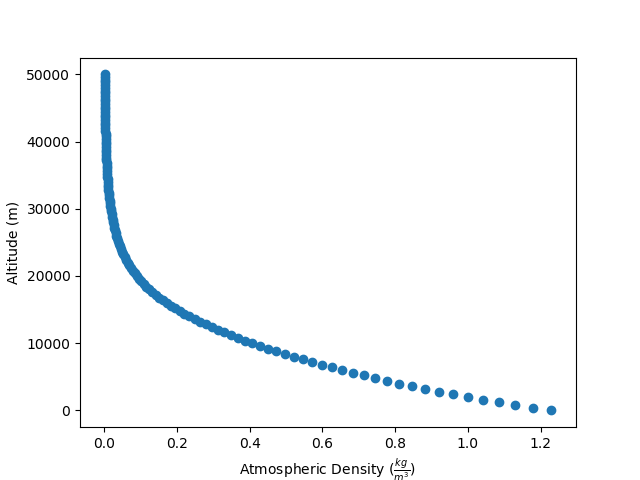
\includegraphics[width=\textwidth]{Images/vertical_density_profile}
        \caption{Vertical Profile of Atmospheric Density}
        \label{density}
    \end{subfigure}
    \hfill
    \begin{subfigure}{.44\textwidth}
        \centering
        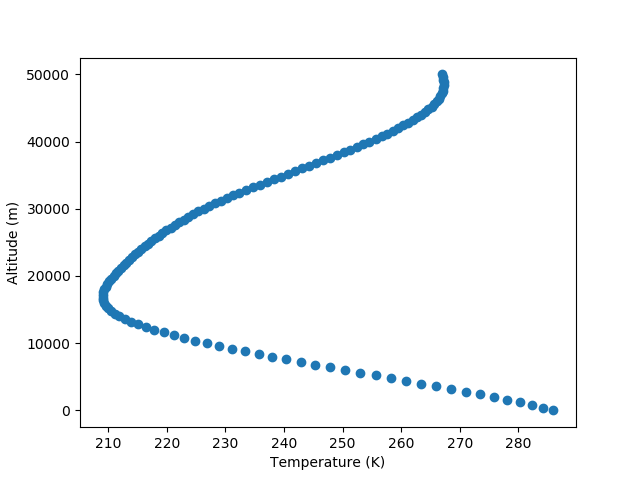
\includegraphics[width=\textwidth]{Images/vertical_temperature_profile.png}
        \caption{Vertical Profile of Temperature}
        \label{temp_profile}
    \end{subfigure}
    \caption{Vertical Profiles of the Troposphere and the Stratosphere}
\end{figure}

\section{Troposphere}
\subsection{Lower and Upper Troposphere}
The troposphere is the layer closest to the surface of the Earth, and rises to a global mean altitude of 11,000 metres. The depth of this layer is relatively thin, however, it contains approximately 80\% of the total overall mass of the atmosphere. 

Because the atmosphere is compressible, air molecules are more compact closer to the surface, thereby increasing the overall atmospheric density and pressure of the air at lower altitudes. Atmospheric pressure just like density decreases exponentially with an increase in altitude (see figure \ref{atmospheric_pressure_intro}). In the lower troposphere, the rate of pressure decrease is about 1000 Pascals for every 100 metres.

\begin{figure}[H]
    \centering
    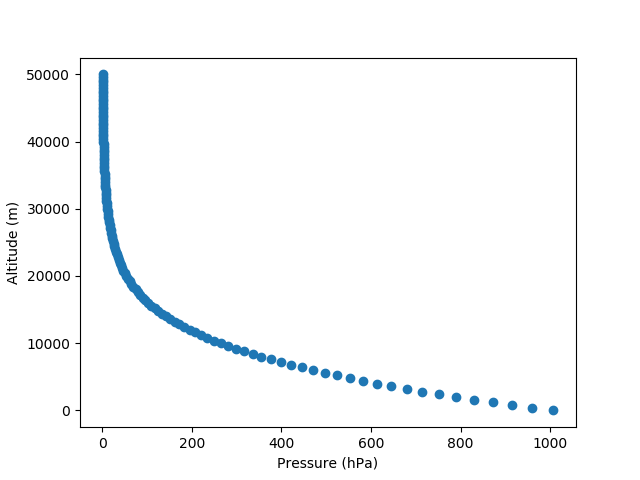
\includegraphics[width=.8\linewidth]{Images/vertical_pressure_profile}
    \caption{Vertical Profile of Atmospheric Pressure in the the Troposphere and the Stratosphere}
    \label{atmospheric_pressure_intro}
\end{figure}

Temperature in the troposphere decreases with altitude (with the exception of the tropopause), contrasting considerably between the lower and upper portions (again, see figure \ref{temp_profile}). Temperature in this particular layer is controlled by a variety of factors, including latitude, season, a location's distance from the ocean, and on, and on. Atmospheric scientists, however, use a concept called a standard atmosphere to present an average atmosphere\cite{temp_in_trop}. The global mean surface temperature is approximately 288.15 K, with the upper portion of the troposphere averaging around 216.65 K. The rate at which this temperature decreases is on average 0.0065 K per metre. Side note, the rate at which temperature increases, decreases, or remains constant on average is commonly called the normal lapse rate by atmospheric scientists.

The mean height of the troposphere varies considerably with latitude. In the tropics, the altitude of the troposphere is around 16,000 metres, but near the poles, this shrinks to about 8,000 metres.

Evidence suggests that the troposphere has undergone a significant rate of warming during the past century. The tropospheric temperature trend in the latter half of the 20th century is estimated at a 0.10 K increase per decade. This is primarily a result of the human-induced perturbation known as, climate change\cite{troposphere}.

\subsection{Tropopause}
At a mean altitude of approximately 11,000 metres, the tropopause commences. This is typically determined by the vertical temperature profile (see figure \ref{temp_profile}). During this particular phase of the atmosphere, temperature remains approximately constant at around 216.65 K until about 32,000 metres above sea level at which point the stratosphere commences. The tropopause is turbulent and well mixed.

\section{Stratosphere}
The stratosphere, as mentioned previously is the second layer of atmosphere. Unlike the troposphere, temperature within the stratosphere increases with altitude. The increasing temperature in the stratosphere is caused by the presence of a layer of ozone near an altitude of approximately 25,000 metres. The ozone molecules absorb high-energy ultraviolet electromagnetic radiation from the sun, which by extension, warms the atmosphere in this layer. The stratosphere is defined as the region between the tropopause and the level at which the maximum warming due to the presence of ozone takes place, which is at an altitude of about 50,000 metres. About 90\% of the ozone in the atmosphere is within this region. Its concentrations in the ozone layer are typically only 1 to 10 parts of ozone per 1 million parts of air\cite{mit}.

\begin{figure}[H]
    \centering
    \chemfig{O=[:50]O \textsuperscript{+}-[:-50]O \textsuperscript{-}}
    \caption{The chemical structure of the ozone atom, $O_3$}
    \label{ozone}
\end{figure}

As mentioned at the beginning of the chapter, the stratosphere consists of extremely dry air, and is by extension, lacking in water vapour. As a consequence, this layer has a low amount of clouds, with almost all clouds being located in the lower, more humid troposphere. This is due to a lack of vertical dynamics within the stratosphere. This also results in materials staying within this layer for long stretches of time. Major meteorite impacts can launch particles straight into the stratosphere attaining extremely high velocities. These particles then linger within this layer, for for months or years, sometimes altering the Earth's global climate significantly\cite{stratosphere}. An example of such an event was the meteorite impact than ultimately killed the dinosaurs. This event launched a significant amount of debris into the stratosphere, which ultimately accumulated, and resulted in a significant drop in global average temperature for the next few years succeeding the event. 

\section{Atmospheric Circulation}
In order for one to truly understand the equations that will be utilised to simulate atmospheric dynamics, it is necessary to examine how atmospheric circulation functions. 

\subsection{Global Heat Energy Budget}
The Global Heat Energy is the equilibrium between incoming and outgoing solar electromagnetic radiation. This incoming and outgoing electromagnetic radiation is known as insolation. 

\begin{definition}
Insolation is defined as the incoming solar electromagnetic radiation that is absorbed, or reflected by the atmosphere
\end{definition}

Approximately 50 \% of the insolation passes through the atmosphere and reaches the surface. Of that, about 46 \% is absorbed with the remainder being reflected. This particular form of reflection is known as the albedo of the Earth. The albedo of an object is just the extent to which that particular object reflects light. Some of the outgoing ultraviolet solar radiation is absorbed by greenhouses gases, such as carbon dioxide and water vapour. This is known as the greenhouse effect. Since the industrial revolution, the amount of greenhouses gases within the atmosphere has dramatically increased. This is resulting in a large amount of this outgoing ultraviolet electromagnetic radiation being absorbed by these greenhouses gases, which ultimately results in the surrounding air being warmed up. This is another example of a human-induced perturbation, as humanity is responsible for the increase in the amount of greenhouses gases within the atmosphere. The insolation that does not reach the surface is either absorbed by the constituent atmospheric gases, or is reflected back into space\cite{insolation}.

\begin{figure}[H]
    \centering
    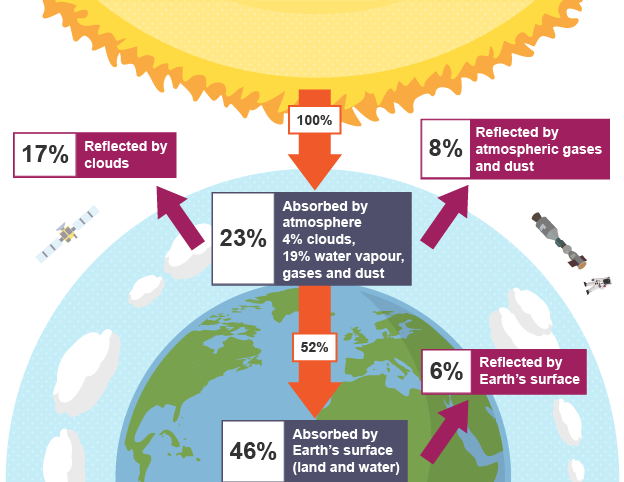
\includegraphics[width=.5\linewidth]{Images/heat_budget.png}
    \caption{The process of insolation within the atmosphere (provided by the BBC)}
\end{figure}

The primary feature of the Earth's thermal energy equilibrium is that there is a net gain of solar radiation in the tropical latitudes and a net loss towards the poles. As evident by figure \ref{energy_balance}, there is a thermal energy deficit between $\pm 35 ^{\circ}$ from the equator and the poles. At these locations, the outgoing radiation exceeds the insolation. Insolation varies wildly depending on the line of latitude at which you are situated; it is as low as approximately $50 J$ at the poles, and peaks at the equator at approximately $275 J$. Terrestrial radiation is less varied, ranging from $120 J$ at the poles to $200 J$ at the equator. 

\begin{figure}[H]
    \centering
    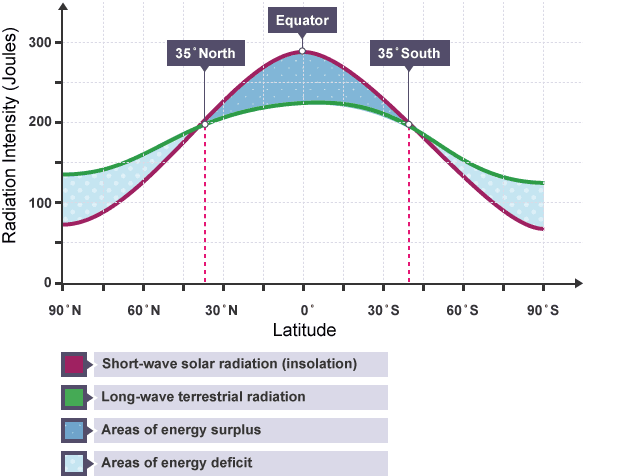
\includegraphics[width=.5\linewidth]{Images/lat_energy_bal.png}
    \caption{Latitude - Radiation Intensity Graph (provided by the BBC)}
    \label{energy_balance}
\end{figure}

Through atmospheric circulation, thermal energy is transferred from areas of low latitude, which have a thermal energy surplus, to areas of high latitude, which have a thermal energy deficit\cite{lat_energy_bal}.

\subsection{Redistrubution of Thermal Energy by Atmospheric Circulation}\label{atmospheric_circulation}
\begin{definition}
Atmospheric circulation is the large-scale movement of air, and together with ocean circulation is the means by which thermal energy is redistributed on the surface of the Earth.
\end{definition}

The atmospheric circulation varies from year to year, but the large-scale structure of its circulation remains fairly constant. A simplified model has been developed in order to explain how the redistrubution of thermal energy from areas of surplus to areas of deficit occurs. It is known as the three-cells model, and can be seen in figure \ref{three_cell}\cite{three_cell}.

\begin{figure}[H]
    \centering
    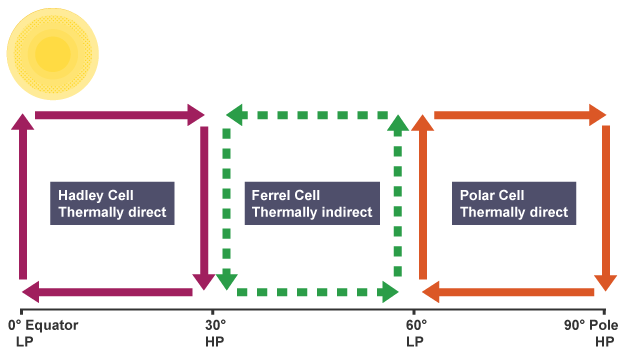
\includegraphics[width=.5\linewidth]{Images/three_cell.png}
    \caption{Three-Cell Atmospheric Circulation Model (provided by the BBC)}
    \label{three_cell}
\end{figure}

Warm air, originating at the equator, ascends creating an area of low pressure, and travels to the 30th parallel, where an area of high pressure is formed. The descended air then travels toward the equator along the surface, replacing the air that rose from the equatorial zone, closing the loop. This is known as the Hadley cell, and it is a closed circulation loop. This atmospheric circulation pattern was developed in an attempt to explain the trade winds, and is considered to be thermally direct; in other words, it exists as a direct consequence of surface temperatures\cite{cells}. As a consequence of this cell, the warmest air does not reach the poles. If atmospheric dynamics were different, however, it is plausible that one large overturning circulation per hemisphere could exist and that wind from the low-latitudes could transport heat to the high-latitudes\cite{hadley_cell}. An eddy is a fluid current whose flow direction differs from that of the general flow.

The Ferrel cell (mid-latitude cell) is located between $30^{\circ}$ and $60^{\circ}$ of latitude. The movement within the Ferrel cell is the reverse of the airflow in the Hadley cell. This cell was the first to account for the westerly winds, more formely known as the `Prevailing Westerlies'. The Ferrell cell is thermally indirect as it is powered by the two other cells. It might be thought of as an eddy created by the Hadley and Polar cells\cite{ferrel}.

The Polar cell is much smaller than the other two cells, and is thermally direct. Similar to the Hadley cell, it operates as a closed circulation loop. As is evident in figure \ref{global_circulation}, cold air sinks at the poles before flowing towards the 60th parallel. Here it is warmed, after which, it rises\cite{cells}. The polar cell, terrain, and Katabatic winds in Antarctica can create very cold conditions at the surface, for instance the lowest temperature recorded on Earth: $183.95 K$ at Vostok Station in Antarctica\cite{polar}.

\begin{figure}[H]
    \centering
    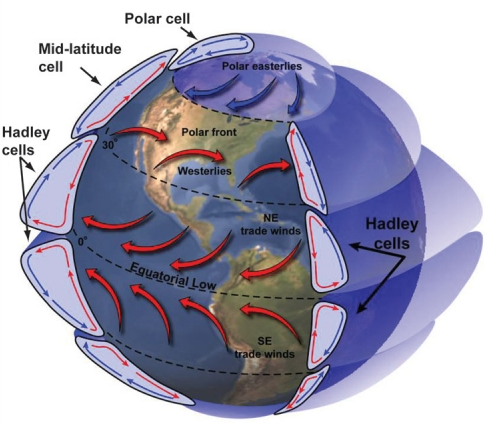
\includegraphics[width=.5\linewidth]{Images/three_cell_globe.png}
    \caption{Idealised Atmospheric Circulation Model (provided by Harvard University)}
    \label{global_circulation}
\end{figure}

The global wind system is created by air blowing from areas of high pressure to areas of low pressure. Winds are affected by the Coriolis effect. In the Northern Hemisphere the Coriolis effect deflects movement to the right and in the Southern Hemisphere it deflects movement to the left.

\section{Ideal Gas Law}\label{ideal}
As mentioned previously, the atmosphere is a continuous stratified fluid with various physical quantities, such as pressure, temperature, and density that characterise its state. Before, one can dive into explaining how one could simulate the dynamics of the atmosphere, it is necessary to briefly touch on the ideal gas equation.

The ideal gas equation is the equation of state for the atmosphere, and is defined as an equation relating temperature, pressure, and specific volume of a system in thermodynamic equilibrium\cite{state_equation}. For most meteorology applications at synoptic scales, it is useful to think of the constituent gases of the atmosphere as ideal gases\cite{ideal_gas}. An ideal gas is an approximation that helps up model and predict the behaviour of real gases. An ideal gas is a hypothetical gas that follows a few rules\cite{iop}: 

\begin{itemize}
    \item The particles of this gas have negligible volume.
    \item The particles of this gas cannot attract, nor repel one another, although they may collide.
    \item Collisions with a surface (i.e. a wall) are elastic.
    \item The motion of the particles in this gas are isotropic. 
\end{itemize}

This idea of an ideal gas forms an equation of state for dry air known as the ideal gas law. This is given by the equation \ref{ideal_gas_law_weird}, or in the form it is more commonly presented in equation \ref{ideal_gas}.

\begin{equation}
    \label{ideal_gas_law_weird}
    p\alpha = RT
\end{equation}

where $\alpha$ is the specific volume.

\begin{equation}
    \label{ideal_gas}
    \Rightarrow p = \rho RT
\end{equation}

It must be noted that there is no gas that is exactly ideal, however, for plenty of gases it is a pretty good approximation. The keen eyed among you may have noticed that it was previously mentioned that stratospheric air is extremely dry. As a result of this, stratospheric air is extremely well described by the ideal gas equation. 

It also must be noted that if the pressure is too large, or the temperature is too low there can be significant deviations from the ideal gas law\cite{ideal_gas}. Considering, however, we are dealing with atmospheric pressure and temperature ranges within the troposphere and the stratosphere, these value extremes will never be reached at any point within them.

\section{Hydrostatic Balance}
\begin{definition}
Hydrostatic Balance describes a balance between vertical pressure gradient and buoyancy forces.
\end{definition}

Another point to examine, before delving into the mathematics of atmospheric dynamics, is to consider a thin horizontal layer of thickness $\Delta z$, as shown in figure \ref{global_circulation}. If we assume that the gas as a whole is at rest, then the layer cannot be gaining or losing momentum. Making note that the pressure is simply the flux of momentum, one can write the vertical momentum budget for the layer as:

\begin{equation}
    p(z) A - p(z + \Delta z) A - A \Delta z \rho g = 0
\end{equation}

\begin{center}
    \begin{tikzpicture}[every edge quotes/.append style={auto, text=black}]
        \pgfmathsetmacro{\cubex}{2}
        \pgfmathsetmacro{\cubey}{2}
        \pgfmathsetmacro{\cubez}{2}
        \draw [draw=black, every edge/.append style={draw=black, densely dashed, opacity=.5}]
        (0,0,0) coordinate (o) -- ++(-\cubex,0,0) coordinate (a) -- ++(0,-\cubey,0) coordinate (b) edge coordinate [pos=1] (g) ++(0,0,-\cubez)  -- ++(\cubex,0,0) coordinate (c) -- cycle
        (o) -- ++(0,0,-\cubez) coordinate (d) -- ++(0,-\cubey,0) coordinate (e) edge (g) -- (c) -- cycle
        (o) -- (a) -- ++(0,0,-\cubez) coordinate (f) edge (g) -- (d) -- cycle;
        
        \draw[->, line width=1.5pt](-0.5,1.65) -- (-0.5,0.65) node[anchor=south west]{$\boldsymbol{p(z + \Delta z) A}$};
        \draw[->, line width=1.5pt](-1,-2.80) -- (-1,-1.80) node[anchor=north west]{$\boldsymbol{p(z) A}$};
        \draw[->, line width=1.5pt](-1,-0.75) node[anchor=south]{$\boldsymbol{A \Delta z \rho g}$} -- (-1,-1.75);
        
        \path [every edge/.append style={draw=black, |-|}]
        (b) +(-5pt,0) coordinate (b2) edge ["$\Delta z$"] (b2 |- a);
    \end{tikzpicture}
\end{center}

which can be rearranged as:

\begin{equation}
    \frac{p(z + \Delta z) - p(z)}{\Delta z} = -\rho g
\end{equation}

and in the $\lim_{\Delta z \to 0}$:

\begin{equation}
    \frac{dp}{dz} = -\rho g
\end{equation}

which is the equation of hydrostatic balance. The key assumption of this equation is that the gas is not accelerating in the vertical. It must be noted that strictly speaking the atmosphere is never in precise hydrostatic balance\cite{iop}. At a synoptic scale, however, it is a pretty reasonable approximation. 


